% !TEX root = ../main.tex
\documentclass[../main.tex]{subfiles}
\begin{document}

\subsection{Examination of volunteer consistency}


\subsection{Disk, Bulge and Bar}

After having obtained aggregated models for our galaxies, we examine the reliability of our models through comparison to other results in the literature. For instance, if we compare the axis ratios of the disks recovered from galaxy builder to the axis ratio of a 2D S\'ersic fit to the r-band SDSS image of each galaxy (as provided in the NASA-Sloan Atlas), we see excellent agreement (Fig.\ref{fig:ax_ratio_comparison}). We note that the results from galaxy builder tend to prefer a slightly more elliptical axis ratio, but plateau at an axis ratio of $0.5$. This could be due to the drawing tool ellipse having a default axis ratio of $0.5$, and biasing volunteer classification or aggregate shapes.

\begin{figure}
  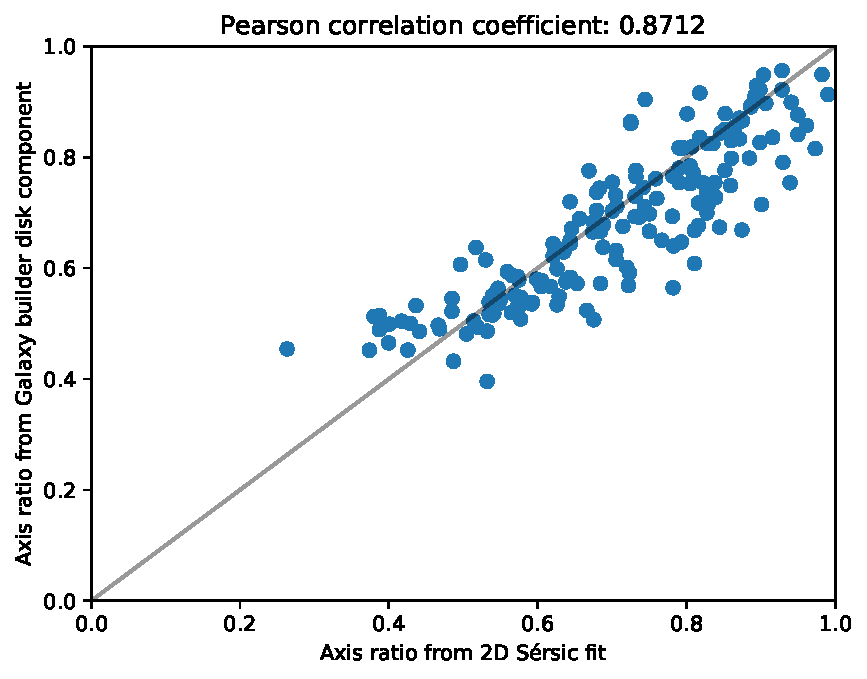
\includegraphics[width=8cm]{images__results/GZBvsNSA_ax-ratio_SERSIC_BA.pdf}
  \caption{Comparison between the axis ratios of the disk components of aggregated Galaxy Builder models to the results of an r-band S\'ersic profile fit.}
  \label{fig:ax_ratio_comparison}
\end{figure}

We can also make comparisons to existing measures of morphology for individual galaxies. Using morphology results from GZ2, we can investigate how likely a volunteer is to incorporate a bulge or bar component in their model relative to its existing morphological classification obtained through citizen science.

Mirroring \citet{Kruk2017:1710.00093v2}, we define a galaxy as disk dominated if the debiased GZ2 fractions $p_\text{no bulge} + p_\text{just noticeable} > p_\text{obvious bulge} + p_\text{dominant bulge}$, or bulge dominated if the converse. Grouping our galaxies based on their type, we find no significant difference in the probability of bulge being present in their model\footnote{The probability of a classification of a disk dominated galaxy having a bulge was \comment{$0.7293 \pm 0.0781$}, whereas for a bulge dominated galaxy it was \comment{$0.7707 \pm 0.0806$}.}. Inspection of resulting aggregated models from galaxy builder suggests that many volunteers were using a highly elliptical bulge component to include both a galaxy's bulge and its bar, it is possible that enforcing a circular bulge may have provided more consistent classifications and less ambiguity for volunteers.

When comparing the probability of a classification containing a bar component against a galaxy being classed as strongly-barred or as having no bar (as defined in \citealt{Masters2010:1003.0449v2}), we see a significant difference: classifications of strongly-barred galaxies ($p_\text{bar} > 0.5$) had a \comment{$0.5713 \pm 0.1549 \%$} chance of containing a bar, vs \comment{$0.3666 \pm 0.1147\%$} for galaxies classed as having no bar ($p_\text{bar} < 0.2$). The Spearman correlation between GZ2's $p_\text{bar}$ and the bar likelihood in galaxy builder is \comment{$0.751$}.

The strongest consistency check of our results is to make comparisons between galaxy builder models and the result of many-component photometric fits. \citet{Kruk2017:1710.00093v2} performed many-component, multi-band decompositions of a selection of Sloan galaxies, 12 of which were also classified in Galaxy Builder. We compare details of those photometric models to the models obtained in Galaxy Builder in table.\ref{table:sandor-fits}. As some of the galaxies received two independent sets of classifications (due to being in the \textit{validation subset}), we list 19 comparisons in the table.

\comment{Some text on the results of the comparison needed (plots?)}

\begin{table*}
  \label{table:sandor-fits}
  \caption{Table comparing the result of guided photometric three-component fits performed by \citet{Kruk2017:1710.00093v2} to the aggregated model obtained from Galaxy Builder. All length units are in arcseconds. \comment{Change from using zooniverse subject ids to IAU name from NSA} \comment{Needs updating}}
  \centering
  \begin{tabular}{lllrrrr}
  Galaxy ID & Model Type & Fit components & $r_\text{eff,disk}$ & $(b / a)_\text{disk}$ & $r_\text{eff,bar}$  & $(b / a)_\text{bar}$ \\
  \hline
  20901993 & Galaxy Builder &  disk+bar+bulge &    15.78 &     0.68 &    7.15 &    0.41 \\
           & Photometric    &        disc+bar &    25.40 &     0.68 &   11.35 &    0.17 \\
  20902000 & Galaxy Builder &      disk+bulge &    21.63 &     0.55 &     NaN &     NaN \\
           & Photometric    &  disc+bar+bulge &    29.71 &     0.58 &   16.21 &    0.21 \\
  20902013 & Galaxy Builder &  disk+bar+bulge &    15.58 &     0.83 &    4.67 &    0.39 \\
           & Photometric    &        disc+bar &    28.33 &     0.89 &    7.45 &    0.14 \\
  20902032 & Galaxy Builder &      disk+bulge &    23.29 &     0.57 &     NaN &     NaN \\
           & Photometric    &        disc+bar &    36.32 &     0.63 &   11.53 &    0.44 \\
  20902040 & Galaxy Builder &  disk+bar+bulge &    22.73 &     0.65 &    9.05 &    0.41 \\
           & Photometric    &        disc+bar &    38.77 &     0.73 &    6.91 &    0.20 \\
  20902049 & Galaxy Builder &      disk+bulge &     8.24 &     0.51 &     NaN &     NaN \\
           & Photometric    &  disc+bar+bulge &    18.66 &     0.73 &    9.46 &    0.35 \\
  20902053 & Galaxy Builder &  disk+bar+bulge &     9.82 &     0.67 &    6.83 &    0.27 \\
           & Photometric    &  disc+bar+bulge &    16.47 &     0.77 &    9.34 &    0.27 \\
  20902057 & Galaxy Builder &      disk+bulge &    10.78 &     0.85 &     NaN &     NaN \\
           & Photometric    &  disc+bar+bulge &    20.31 &     0.96 &   15.41 &    0.22 \\
  20902058 & Galaxy Builder &      disk+bulge &    14.68 &     0.89 &     NaN &     NaN \\
           & Photometric    &  disc+bar+bulge &    24.88 &     0.94 &    5.62 &    0.20 \\
  20902064 & Galaxy Builder &  disk+bar+bulge &    13.85 &     0.63 &    7.93 &    0.29 \\
           & Photometric    &        disc+bar &    17.16 &     0.84 &   13.68 &    0.20 \\
  21686510 & Galaxy Builder &      disk+bulge &    18.89 &     0.52 &     NaN &     NaN \\
           & Photometric    &  disc+bar+bulge &    29.71 &     0.58 &   16.21 &    0.21 \\
  21686523 & Galaxy Builder &  disk+bar+bulge &    16.60 &     0.67 &    7.90 &    0.38 \\
           & Photometric    &        disc+bar &    33.31 &     0.76 &    9.86 &    0.27 \\
  21686542 & Galaxy Builder &  disk+bar+bulge &    15.30 &     0.87 &    6.76 &    0.56 \\
           & Photometric    &        disc+bar &    28.33 &     0.89 &    7.45 &    0.14 \\
  21686549 & Galaxy Builder &             bar &      NaN &      NaN &    6.56 &    0.32 \\
           & Photometric    &        disc+bar &    43.44 &     0.75 &   11.09 &    0.48 \\
  21686569 & Galaxy Builder &  disk+bar+bulge &    24.52 &     0.72 &    9.98 &    0.40 \\
           & Photometric    &        disc+bar &    38.77 &     0.73 &    6.91 &    0.20 \\
  21686578 & Galaxy Builder &           bulge &      NaN &      NaN &     NaN &     NaN \\
           & Photometric    &  disc+bar+bulge &    18.66 &     0.73 &    9.46 &    0.35 \\
  21686582 & Galaxy Builder &  disk+bar+bulge &    10.17 &     0.70 &    6.61 &    0.26 \\
           & Photometric    &  disc+bar+bulge &    16.47 &     0.77 &    9.34 &    0.27 \\
  21686587 & Galaxy Builder &  disk+bar+bulge &    15.62 &     0.89 &    6.08 &    0.35 \\
           & Photometric    &  disc+bar+bulge &    24.88 &     0.94 &    5.62 &    0.20 \\
  21686593 & Galaxy Builder &  disk+bar+bulge &    13.47 &     0.62 &    9.25 &    0.23 \\
           & Photometric    &        disc+bar &    17.16 &     0.84 &   13.68 &    0.20 \\
  \hline
  \end{tabular}
\end{table*}

% \comment{Compare bulge / disk ratio?}

% \comment{Pbar vs number of bars drawn}

% \comment{Pspiral vs frequency of classification having spiral arms}


\subsection{Spiral Arms}

In order to benchmark the reliability of this method of spiral parameter extraction, we compare the result of our logarithmic spiral fit to the relationship obtained by \citet{Hart2016:1607.01019v1} between GZ2 classification and galaxy pitch angle (Fig.\ref{fig:hart_pitch_angle}). Their fit was obtained using a leading automated spiral arm detection and fitting tool, \textsc{SpArcFiRe} \citep{Davis2014:1402.1910v1}. We find good agreement, though the large error bars on the GZ2-produced pitch angle (along with the caveat in the paper that these pitch angles should not be used for individual galaxies) make this comparison rather inconclusive.

\begin{figure}
  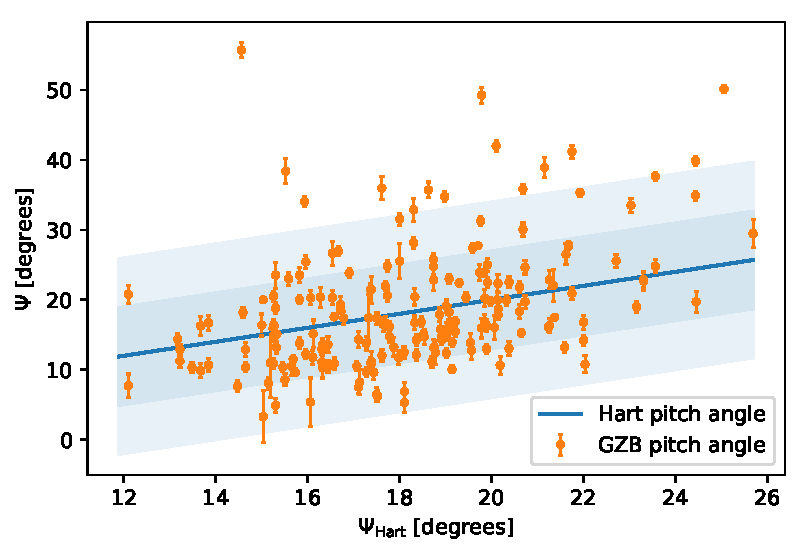
\includegraphics[width=8cm]{images__results/pitch-angle-comparison.pdf}
  \caption{A comparison of Pitch angle obtained by \citet{Hart2016:1607.01019v1} with measured pitch angles for the aggregated model results in galaxies in the Galaxy Zoo Builder sample. Errors on the Galaxy Builder pitch angles come from dispersion in the arms drawn by volunteers.}
  \label{fig:hart_pitch_angle}
\end{figure}

We can also directly compare the pitch angles from Galaxy Builder models to the output of the SpArcFiRe software, as shown in Fig.\ref{fig:sparcfire_pitch_angle}. The SpArcFiRe pitch angle used is the length-weighted mean of all arms of the dominant chirality of a galaxy.

\begin{figure}
  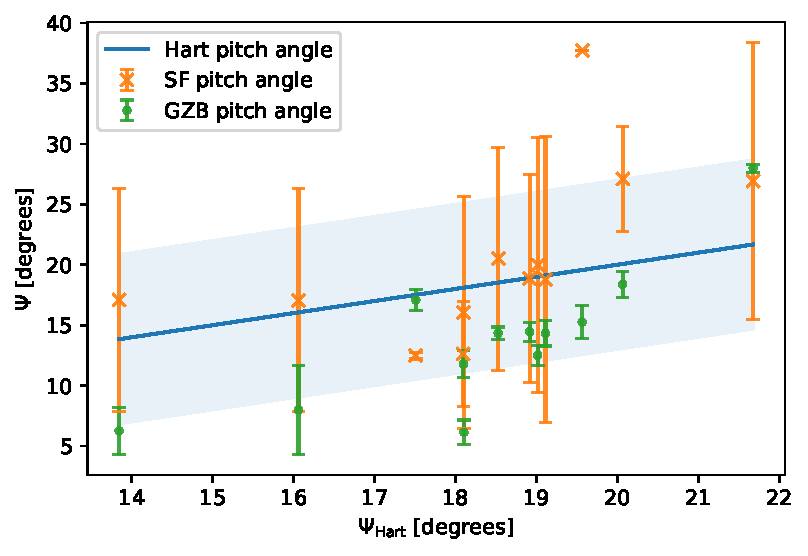
\includegraphics[width=8cm]{images__results/pitch-angle-comparison2.pdf}
  \caption{A comparison between pitch angles obtained by \citet{Hart2016:1607.01019v1} (blue line) to those obtained through Galaxy Builder (orange) and SpArcFiRe (green). It is worth noting that in this plot, unlike Fig.\ref{fig:hart_pitch_angle}, errors are the sample error of arms used in the averaging and is a measure of inter-arm variation pitch angle.}
  \label{fig:sparcfire_pitch_angle}
\end{figure}

\comment{Show results of sparcfire / GZ2 comparison}

\subsubsection{Model selection}

\comment{This is more "Are log spirals right?", should it go in a different paper?}

Group K-fold cross validation is used to perform model selection, where points are grouped according to the poly-line they were drawn in. Five folds is chosen as a compromise to minimise variance on the resulting scores, while also minimising the bias from removing too many classifications from our training set. To score the goodness-of-fit of a model, we use negative median absolute error.


In order to confidently describe a spiral arm as not a logarithmic spiral, we \comment{TODO}

\end{document}
